\documentclass[crop,tikz,10pt]{standalone}

\usepackage{tikz}
\usetikzlibrary{calc}
\usetikzlibrary{arrows.meta}
\usetikzlibrary{decorations.text}
\usetikzlibrary{backgrounds}

\definecolor{bg1}{RGB}{244,231,195}
\definecolor{bg2}{RGB}{234,204,161}
\definecolor{l1}{RGB}{209,148,106}

\begin{document}

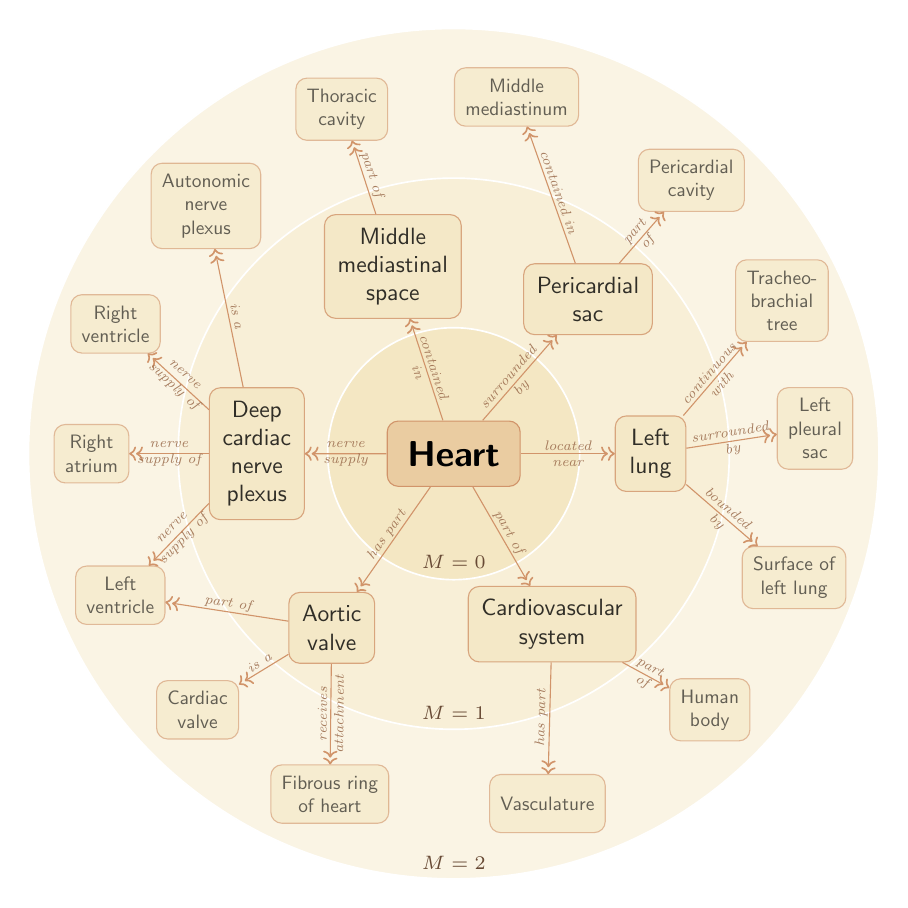
\begin{tikzpicture}[
    font=\sffamily,
    l/.style={
        line width=0.4pt,
        color=l1,
        -{Computer Modern Rightarrow[line width=0.6pt] . Computer Modern Rightarrow[line width=0.6pt]}
    },
    none/.style={
        opacity=0
    },
    e/.style={
        rounded corners, align=center,
        minimum height=3em,
        minimum width=3em,
        inner sep=1.3ex,
        fill=bg1,
        draw=l1,
        line width=0.4pt
    },
    l1/.style={
        minimum height=0,
        scale=1.3,
        font=\bfseries\sffamily,
        fill=bg2
    },
    l2/.style={scale=0.85,opacity=0.80},
    l3/.style={scale=0.70,opacity=0.60},
    l4/.style={scale=0.50,opacity=0.40},
    p/.style={
        font=\tiny\itshape, align=center,
        sloped, shape=rectangle, color=l1!75!black, opacity=0.9
    },
    p1/.style={
        p,
        above=3pt,
        anchor=center
    },
    p2/.style={
        p
    },
    r/.style={
        font=\scriptsize,
        color=l1!50!black,
        anchor=south
    }
]
    
    \node [e,l1] (hea) at (0, 0) {Heart};
    
    \node [e,l2] (lun) at (0:2.5) {Left\\lung};
    \node [e,l2] (per) at (49:2.6) {Pericardial\\sac};
    \node [e,l2] (spa) at (108:2.5) {Middle\\mediastinal\\space};
    \node [e,l2] (dcn) at (180:2.5) {Deep\\cardiac\\nerve\\plexus};
    \node [e,l2] (val) at (235:2.7) {Aortic\\valve};
    \node [e,l2] (sys) at (300:2.5) {Cardiovascular\\system};
    
    \draw (hea) edge [l] node [p2] {located\\near} (lun);
    \draw (hea) edge [l] node [p2,pos=0.44] {surrounded\\by} (per);
    \draw (hea) edge [l] node [p2] {contained\\in} (spa);
    \draw (hea) edge [l] node [p2] {nerve\\supply} (dcn);
    \draw (hea) edge [l] node [p1] {has part} (val);
    \draw (hea) edge [l] node [p1] {part of} (sys);
    
    \node [e,l3] (sll) at (-20:4.6) {Surface of\\left lung};
    \node [e,l3] (lps) at (  4:4.6) {Left\\pleural\\sac};
    \node [e,l3] (tre) at ( 25:4.6) {Tracheo-\\brachial\\tree};
    \node [e,l3] (cav) at ( 49:4.6) {Pericardial\\cavity};
    \node [e,l3] (med) at ( 80:4.6) {Middle\\mediastinum};
    \node [e,l3] (thx) at (108:4.6) {Thoracic\\cavity};
    \node [e,l3] (anp) at (135:4.45) {Autonomic\\nerve\\plexus};
    \node [e,l3] (rvn) at (159:4.6) {Right\\ventricle};
    \node [e,l3] (rat) at (180:4.6) {Right\\atrium};
    \node [e,l3] (lvn) at (203:4.6) {Left\\ventricle};
    \node [e,l3] (cvl) at (225:4.6) {Cardiac\\valve};
    \node [e,l3] (frh) at (250:4.6) {Fibrous ring\\of heart};
    \node [e,l3] (vas) at (285:4.6) {Vasculature};
    \node [e,l3] (bod) at (315:4.6) {Human\\body};
    
    \draw (lun) edge [l] node [p2] {bounded\\by} (sll);
    \draw (lun) edge [l] node [p2] {surrounded\\by} (lps);
    \draw (lun) edge [l] node [p2] {continuous\\with} (tre);
    \draw (per) edge [l] node [p2] {part\\of} (cav);
    \draw (per) edge [l] node [p1] {contained in} (med);
    \draw (spa) edge [l] node [p1] {part of} (thx);
    \draw (dcn) edge [l] node [p1] {is a} (anp);
    \draw (dcn) edge [l] node [p2] {nerve\\supply of} (lvn);
    \draw (dcn) edge [l] node [p2] {nerve\\supply of} (rat);
    \draw (dcn) edge [l] node [p2] {nerve\\supply of} (rvn);
    \draw (val) edge [l] node [p1] {part of} (lvn);
    \draw (val) edge [l] node [p1] {is a} (cvl);
    \draw (val) edge [l] node [p2] {receives\\attachment} (frh);
    \draw (sys) edge [l] node [p1] {has part} (vas);
    \draw (sys) edge [l] node [p2] {part\\of} (bod);
    
    % \node  (o00) at ( -2:6) {};
    % \node  (o01) at (  9:6) {};
    % \node  (o02) at ( 20:6) {};
    % \node  (o03) at ( 30:6) {};
    % \node  (o04) at ( 43:6) {};
    % \node  (o05) at ( 55:6) {};
    % \node  (o06) at ( 69:6) {};
    % \node  (o07) at ( 81:6) {};
    % \node  (o08) at ( 93:6) {};
    % \node  (o09) at (104:6) {};
    % \node  (o10) at (116:6) {};
    % \node  (o11) at (132:6) {};
    % \node  (o12) at (144:6) {};
    % \node  (o13) at (152:6) {};
    % \node  (o14) at (164:6) {};
    % \node  (o15) at (180:6) {};
    % \node  (o16) at (198:6) {};
    % \node  (o17) at (210:6) {};
    % \node  (o18) at (218:6) {};
    % \node  (o19) at (228:6) {};
    % \node  (o20) at (240:6) {};
    % \node  (o21) at (252:6) {};
    % \node  (o22) at (272:6) {};
    % \node  (o23) at (282:6) {};
    % \node  (o24) at (292:6) {};
    % \node  (o25) at (302:6) {};
    % \node  (o26) at (312:6) {};
    % \node  (o27) at (324:6) {};
    % \node  (o28) at (336:6) {};
    % \node  (o29) at (348:6) {};
    
    % \draw (lps) edge [none] (o00);
    % \draw (lps) edge [none] (o01);
    % \draw (tre) edge [none] (o02);
    % \draw (tre) edge [none] (o03);
    % \draw (cav) edge [none] (o04);
    % \draw (cav) edge [none] (o05);
    % \draw (med) edge [none] (o06);
    % \draw (med) edge [none] (o07);
    % \draw (med) edge [none] (o08);
    % \draw (thx) edge [none] (o09);
    % \draw (thx) edge [none] (o10);
    % \draw (anp) edge [none] (o11);
    % \draw (anp) edge [none] (o12);
    % \draw (rvn) edge [none] (o13);
    % \draw (rvn) edge [none] (o14);
    % \draw (rat) edge [none] (o15);
    % \draw (lvn) edge [none] (o16);
    % \draw (lvn) edge [none] (o17);
    % \draw (cvl) edge [none] (o18);
    % \draw (cvl) edge [none] (o19);
    % \draw (frh) edge [none] (o20);
    % \draw (frh) edge [none] (o21);
    % \draw (vas) edge [none] (o22);
    % \draw (vas) edge [none] (o23);
    % \draw (vas) edge [none] (o24);
    % \draw (vas) edge [none] (o25);
    % \draw (bod) edge [none] (o26);
    % \draw (bod) edge [none] (o27);
    % \draw (sll) edge [none] (o28);
    % \draw (sll) edge [none] (o29);
    
    \node [r,yshift=0.5pt] at (270:1.6) {$M=0$};
    \node [r] at (270:3.5) {$M=1$};
    \node [r] at (270:5.4) {$M=2$};
    
    \begin{scope}[on background layer]
        % \fill [draw=white,fill=bg1!40!white,line width=0.6pt] (hea) circle (7);
        \fill [draw=white,fill=bg1!45!white,line width=0.6pt] (hea) circle (5.4);
        \fill [draw=white,fill=bg1!67!white,line width=0.6pt] (hea) circle (3.5);
        \fill [draw=white,fill=bg1!100!white,line width=0.6pt] (hea) circle (1.6);
    \end{scope}
    
\end{tikzpicture}

\end{document}
